\section{Results}
\label{sec:results}
% Figures of the results section, drawn from the files in docs/latex/data.

\newcommand{\figpath}{%
\begin{figure}[htbp]
  \centering
  \begin{tikzpicture}[x=3.3cm, y=3.3cm]
    \arenaplan
    \arenaobstacles{2.10/0.45, 1.60/0.10, 2.00/-0.35}
    \draw[cA, line width=0.5pt, line join=round] plot file {../data/track_m03.dat};
    \draw[draw=ink, fill=panel] (-0.017,-0.075) rectangle (0.163,0.075);
    \draw[|-|] (2.3,-0.72) -- (3.3,-0.72);
    \node[note, below] at (2.8,-0.73) {1\,m};
  \end{tikzpicture}
  \caption{True path of the robot in run 3 (obstacle preset b, three boxes). The path
  follows the entry line, visits the three drop zones, and then alternates between the pick
  bays and the drop zones, passing the boxes on whichever side the planner finds free.}
  \label{fig:path}
\end{figure}}

\newcommand{\figtimes}{%
\begin{figure}[htbp]
  \centering
  \begin{tikzpicture}
    \begin{axis}[report, ybar stacked, bar width=9pt, ymin=0, ymax=340,
        xlabel={run}, ylabel={simulated time [s]}, xtick={1,...,12}, enlarge x limits=0.06,
        area legend, grid=none, ymajorgrids]
      \addplot[fill=cD!55, draw=cD] table[x expr=\coordindex+1, y=t_line, col sep=comma] {../data/runs.csv};
      \addplot[fill=cA, draw=cA] table[x expr=\coordindex+1, y=t_survey, col sep=comma] {../data/runs.csv};
      \addplot[fill=cB!70, draw=cB] table[x expr=\coordindex+1, y=t_coins, col sep=comma] {../data/runs.csv};
      \legend{entry line, survey of drop zones, three coins}
    \end{axis}
  \end{tikzpicture}
  \caption{Duration of the three parts of the mission in each run.}
  \label{fig:times}
\end{figure}}

\newcommand{\figslam}{%
\begin{figure}[htbp]
  \centering
  \begin{tikzpicture}
    \begin{axis}[report, xlabel={simulated time [s]}, ylabel={position error [mm]},
        xmin=0, xmax=310, ymin=0, ymax=45, legend columns=-1]
      \addplot[cA, line width=0.6pt] table[x=t, y=err_mm] {../data/slam_m03.dat};
      \addplot[cB, line width=0.6pt] table[x=t, y=odom_mm] {../data/slam_m03.dat};
      \legend{map pose, odometry alone}
    \end{axis}
  \end{tikzpicture}
  \caption{Distance between the estimated and the true position of the robot in run 3, for
  the pose in the map and for the odometry filter alone.}
  \label{fig:slam}
\end{figure}}

\newcommand{\figdock}{%
\begin{figure}[htbp]
  \centering
  \begin{subfigure}[b]{0.48\linewidth}
    \centering
    \begin{tikzpicture}
      \begin{axis}[report, width=\linewidth, height=0.9\linewidth,
          xlabel={across the stem [mm]}, ylabel={along the stem [mm]},
          xmin=-10, xmax=10, ymin=-10, ymax=10, axis equal image]
        \fill[black!25] (axis cs:-10,-6) rectangle (axis cs:10,6);
        \addplot[only marks, mark=*, mark size=1.3pt, cA]
          table[x=lateral_mm, y=along_mm, col sep=comma] {../data/picks.csv};
      \end{axis}
    \end{tikzpicture}
    \caption{Array centre when the jaws close}
  \end{subfigure}\hfill
  \begin{subfigure}[b]{0.48\linewidth}
    \centering
    \begin{tikzpicture}
      \begin{axis}[report, width=\linewidth, height=0.9\linewidth,
          xlabel={along the stem [mm]}, ylabel={across the stem [mm]},
          xmin=-25, xmax=25, ymin=-25, ymax=25, axis equal image]
        \addplot[only marks, mark=*, mark size=1.3pt, cB]
          table[x=dx_mm, y=dy_mm, col sep=comma] {../data/drops.csv};
      \end{axis}
    \end{tikzpicture}
    \caption{Coin after release}
  \end{subfigure}
  \caption{Docking accuracy over all picks and drops. (a) Position of the centre of the
  infrared array relative to the centre of the crossbar at the moment the jaws close; the
  grey band is the crossbar, 12\unit{mm} wide. (b) Final position of each coin relative to
  the centre of its drop square, which extends to $\pm125\unit{mm}$.}
  \label{fig:dock}
\end{figure}}

\newcommand{\figline}{%
\begin{figure}[htbp]
  \centering
  \begin{tikzpicture}
    \begin{axis}[report, width=0.8\linewidth, height=0.36\linewidth,
        xlabel={distance along the arena, $x$ [m]}, ylabel={offset from the line [mm]},
        xmin=0, xmax=1.45, ymin=-12, ymax=12, legend columns=-1]
      \addplot[cD, line width=0.6pt] table[x=x, y=err_mm] {../data/line_n0.0_v0.10.dat};
      \addplot[cA, line width=0.6pt] table[x=x, y=err_mm] {../data/line_n0.05_v0.10.dat};
      \addplot[cB, line width=0.6pt] table[x=x, y=err_mm] {../data/line_n1.0_v0.10.dat};
      \legend{no noise, 0.05\,V, 1.0\,V}
    \end{axis}
  \end{tikzpicture}
  \caption{Offset of the array centre from the entry line at 0.10\unit{m/s}, for three
  levels of noise on the infrared readings. The two arcs of the S-bend lie between
  $x=0.15$ and $1.19\unit{m}$.}
  \label{fig:line}
\end{figure}}


All results in this section were obtained in the simulation of \cref{sec:simulation}, in
the arena of \cref{sec:arena}, with the parameters of \cref{app:parameters}. Times are
simulated time. Positions called true are the ground truth of the simulator.

\subsection{Method}
The mission was run twelve times without a display: three runs for each of the four
obstacle layouts (none and the presets a, b and c), with a different combination of pick
order and drop order in almost every run (\cref{tab:runs}). All runs used the same map,
built once in the empty arena, and the same start pose. The noise on the infrared readings
was 0.05\unit{V}. Each run was recorded as described in \cref{sec:verification} and scored
by the referee.

\subsection{Outcome of the Mission}
All twelve runs passed: in every run the referee found all three coins inside the drop
squares of their colours, 36 coins of 36. No station needed a second attempt, no QR code
was missed, and the navigation entered no recovery behaviour in any run.

\begin{table}[htbp]
  \centering
  \caption{The twelve mission runs. Pick and drop give the colours of bays 1 to 3 and of
  drop zones 1 to 3. Map error is the RMS distance between the pose in the map and the true
  pose; line error is the RMS offset of the array from the entry line.}
  \label{tab:runs}
  \begin{tabular}{@{}cccccccc@{}}
    \toprule
    Run & Pick & Drop & Obstacles & Coins home & Time [s] & Path [m] & Map error [mm] \\
    \midrule
    1 & RGB & BRG & a & 3 of 3 & 301 & 18.4 & 8.4 \\
    2 & RGB & BRG & none & 3 of 3 & 300 & 18.0 & 8.8 \\
    3 & GBR & RGB & b & 3 of 3 & 307 & 18.7 & 10.7 \\
    4 & BRG & GRB & c & 3 of 3 & 305 & 17.9 & 10.6 \\
    5 & RBG & RGB & none & 3 of 3 & 299 & 17.7 & 11.8 \\
    6 & GRB & BGR & a & 3 of 3 & 299 & 18.4 & 11.8 \\
    7 & BGR & RBG & b & 3 of 3 & 304 & 18.6 & 9.2 \\
    8 & RGB & GBR & c & 3 of 3 & 292 & 17.6 & 10.0 \\
    9 & GBR & BRG & none & 3 of 3 & 298 & 17.5 & 9.7 \\
    10 & BRG & RGB & a & 3 of 3 & 295 & 17.8 & 9.8 \\
    11 & RBG & GRB & b & 3 of 3 & 300 & 18.5 & 9.7 \\
    12 & GRB & RBG & c & 3 of 3 & 298 & 17.6 & 8.2 \\
    \bottomrule
  \end{tabular}
\end{table}

A mission takes 300\unit{s} on average, between 293 and 307\unit{s} (\cref{fig:times}): 19\unit{s}
on the entry line, 83\unit{s} for the survey of the three drop zones and 198\unit{s} for the
three coins, or 66\unit{s} per coin. The robot covers 18.1\unit{m}, which is an average of
0.06\unit{m/s}; most of the time goes into turning on the spot, the slow approach along the
stems and the waiting for the jaws and for the QR codes. The obstacles cost little. The
mean time is 299\unit{s} without obstacles and 304\unit{s} with the three boxes of
preset b, and the paths differ by less than a metre. \Cref{fig:path} shows the true path of
one run.

\figpath
\figtimes

\subsection{Line Following}
\label{sec:res-line}
On the entry line of the twelve missions, the centre of the array stayed within 6.0\unit{mm}
of the centre of the line, with an RMS offset of 1.6\unit{mm} (1.4 to 2.1\unit{mm} over the
runs). The line is 12\unit{mm} wide and the channels are 15\unit{mm} apart, so the offset is
a tenth of the pitch: the interpolation between partially covered channels
(\cref{eq:offset}) works as intended. In every run the array stopped on the start square.

The line follower was also run on its own on the entry line, once for each of several noise
levels and speeds (\cref{tab:line,fig:line}). Two results stand out. The follower is
insensitive to noise up to 0.2\unit{V}, four times the level used in the missions, because
readings below the floor threshold carry no weight. At 0.5\unit{V} noise crosses that
threshold and the offset grows fourfold, and at 1.0\unit{V} it reaches 46\unit{mm}, close
to the half span of the array, although the line was not lost. And the offset grows quickly
with speed: 1.1\unit{mm} at the docking speed, 1.7\unit{mm} at the entry speed, and
17.6\unit{mm} at 0.30\unit{m/s}. This agrees in direction with \cref{eq:line-dynamics},
where the damping ratio falls with the square root of the speed, from 0.72 at
0.05\unit{m/s} to 0.29 at 0.30\unit{m/s}. The speeds chosen for the mission are on the
well-damped side.

\begin{table}[htbp]
  \centering
  \caption{Line follower alone on the entry line, one run per row. Offset of the array
  centre from the centre of the line.}
  \label{tab:line}
  \begin{tabular}{@{}ccccc@{}}
    \toprule
    Noise [V] & Speed [m/s] & RMS offset [mm] & Largest offset [mm] & Start square reached \\
    \midrule
    0 & 0.10 & 1.5 & 4.0 & yes \\
    0.05 & 0.10 & 1.7 & 4.3 & yes \\
    0.2 & 0.10 & 1.9 & 4.1 & yes \\
    0.5 & 0.10 & 6.8 & 19.7 & yes \\
    1.0 & 0.10 & 18.0 & 45.9 & yes \\
    \midrule
    0.05 & 0.05 & 1.1 & 2.8 & yes \\
    0.05 & 0.15 & 3.3 & 7.7 & yes \\
    0.05 & 0.20 & 7.4 & 16.3 & yes \\
    0.05 & 0.30 & 17.6 & 37.9 & yes \\
    \bottomrule
  \end{tabular}
\end{table}

\figline

\subsection{Localisation}
\label{sec:res-slam}
Over the part of each mission that is driven in the room, the pose in the map differed
from the true pose by 9.9\unit{mm} RMS (8.2 to 11.8\unit{mm} over the runs). The 95th
percentile was 19\unit{mm} on average, the largest error in any run 39\unit{mm}, and the
heading error 0.7\unit{^\circ} RMS. These errors are below the goal tolerance of the
navigation, 20\unit{mm}, for most of the time, and well below the lateral error that a stem
can absorb.

This result has to be read with a second one (\cref{fig:slam}). The odometry filter alone,
without any correction from the map, was never more than 30\unit{mm} from the truth in any
run, and ended a mission of 18\unit{m} with an error of 16\unit{mm} on average. In this
simulation the odometry is nearly ideal: the encoders have no quantisation, the floor is
uniform and the drive stays inside its traction limit. The map therefore has little to
correct, and its corrections are of the same size as the error they remove. The runs show
that the localisation is stable over five minutes and does not jump, which was the failure
described in \cref{sec:slam}; they do not show how much it would contribute on a real
floor, where wheel odometry drifts.

\figslam

\subsection{Docking}
\label{sec:res-dock}
\Cref{fig:dock} gives the accuracy of the two movements on which the manipulation depends,
over all 36 picks and 36 drops.

\paragraph{Pick.} At the moment the jaws closed, the centre of the array was 2.7\unit{mm}
RMS to the side of the stem, with a largest offset of 7.1\unit{mm}, and on average
2.9\unit{mm} past the centre of the crossbar (0.9 to 6.0\unit{mm}), that is, always on the
bar. The heading differed from the direction of the stem by 2.9\unit{^\circ} RMS and by
7.1\unit{^\circ} at most. The heading is the least well controlled quantity: a stem of
0.30\unit{m} removes a lateral error faster than it removes the turn that the correction
itself introduces. All 36 coins were nevertheless caged, which is the tolerance that the
shape of the jaws was designed to provide.

\paragraph{Drop.} The coins came to rest 9.0\unit{mm} from the centres of their squares on
average and 20.7\unit{mm} at most. The square extends 125\unit{mm} from its centre, so the
margin is a factor of six. The offsets are not centred: every coin lies between 5 and
11\unit{mm} short of the centre along the stem, which is the distance by which the coin
sits further back between the jaws than the nominal 0.13\unit{m}.

\figdock

\subsection{The Simulated Robot}
\Cref{fig:sim-shots} shows the simulation during a mission.

\begin{figure}[htbp]
  \centering
  \begin{subfigure}[b]{0.49\linewidth}
    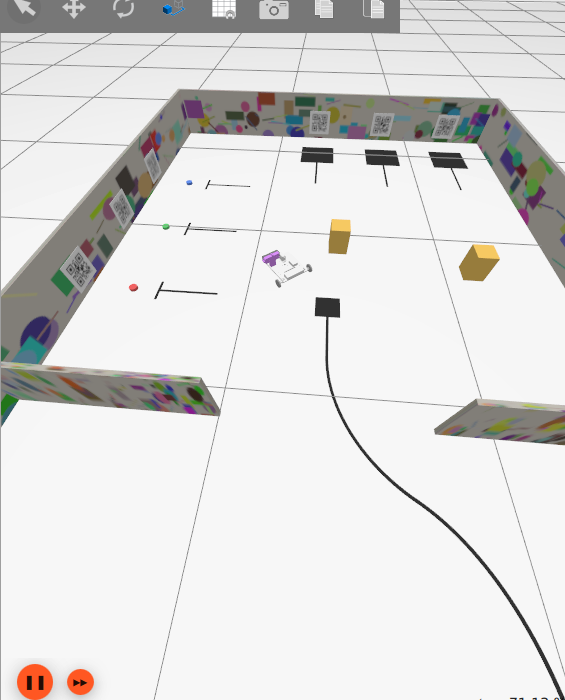
\includegraphics[width=\linewidth]{sim_arena.png}
    \caption{Entry line and room in Gazebo}
  \end{subfigure}\hfill
  \begin{subfigure}[b]{0.49\linewidth}
    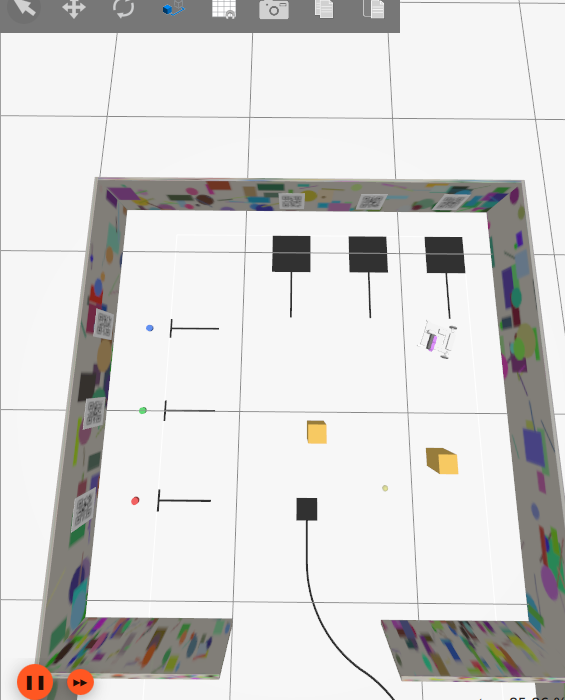
\includegraphics[width=\linewidth]{sim_pick.png}
    \caption{Robot in the room, seen from above the entry lane}
  \end{subfigure}\\[4pt]
  \begin{subfigure}[b]{0.8\linewidth}
    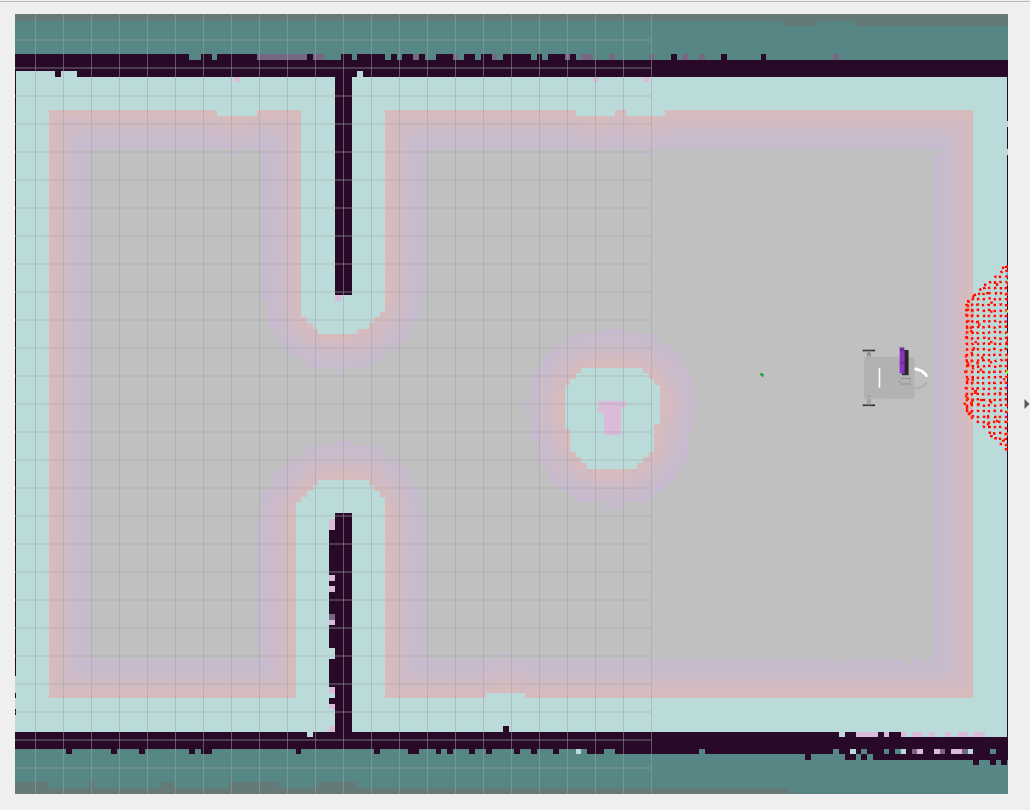
\includegraphics[width=\linewidth]{sim_rviz.png}
    \caption{Map and inflated costmap in RViz, with the robot at a drop zone}
  \end{subfigure}
  \caption{The simulated mission.}
  \label{fig:sim-shots}
\end{figure}

\subsection{Summary}
\begin{itemize}
  \item The mission succeeded in twelve of twelve runs, with four obstacle layouts and
        eleven combinations of colours, in 300\unit{s} on average.
  \item The line follower holds the line within 6\unit{mm} at the speeds used, tolerates
        four times the nominal sensor noise, and degrades with speed as the analysis of its
        damping predicts.
  \item The pose in the map is accurate to 10\unit{mm} RMS, but the simulated odometry is
        nearly as good, so the simulation does not test the value of the map.
  \item The robot stops on a crossbar within 7\unit{mm} laterally and places coins within
        21\unit{mm} of the centre of a square of 250\unit{mm}.
\end{itemize}
